% LaTeX source for ``Algorithms for Computer Simulation of Molecular Systems''
% Copyright (c) 2023 รังสิมันต์ เกษแก้ว (Rangsiman Ketkaew).

% License: Creative Commons Attribution-NonCommercial-NoDerivatives 4.0 International (CC BY-NC-ND 4.0)
% https://creativecommons.org/licenses/by-nc-nd/4.0/

\chapter{พลวัตเชิงโมเลกุลแบบดั้งเดิม}
\label{ch:md}

%----------------------------------------
\section{การประยุกต์ใช้ Molecular Dynamics}
%----------------------------------------

ก่อนที่เราจะไปศึกษาวิธีการจำลองระบบโมเลกุลที่มีความซับซ้อนนั้นเราควรเริ่มต้นด้วยการศึกษาวิธีอย่างง่ายก่อนนั่นก็คือ Molecular Dynamics (MD)
(จริง ๆ จะว่าไปแล้ววิธีนี้ก็ไม่ได้ง่ายนะครับ ถ้าลงรายละเอียดลึก ๆ แล้วก็มีความซับซ้อนมากพอสมควร ซึ่งในปัจจุบันนั้นก็มีการทำวิจัยที่เกี่ยวข้องกับ%
การพัฒนาเทคนิคของวิธี MD อย่างต่อเนื่อง) เราใช้เทคนิคการจำลองทางคอมพิวเตอร์ในการทำความเข้าใจคุณสมบัติของระบบที่ประกอบไปด้วยโมเลกุล
ๆ โมเลกุลในเชิงโครงสร้างและอันตรกิริยาในระดับจุลภาคหรือหน่วยย่อย ซึ่งหน่วยย่อยในที่นี้ก็คือโมเลกุลนั่นเอง โดยเราสามารถแบ่งวิธีการจำลองออก%
ได้เป็น 2 วิธีคือ Molecular Dynamics (MD) กับ Monte Carlo (MC) และหนังสือเล่มนี้จะเน้นไปที่ MD ซึ่งเป็นวิธีที่สามารถนำมาใช้ในการศึกษา%
คุณสมบัติเชิงพลวัตได้ เช่น สัมประสิทธิ์การเคลื่อนที่ (Transport Coefficients), การตอบสนองต่อการรบกวนแบบที่ขึ้นกับเวลา (Time-dependt
Response to Perturbation), และสเปกตรัม

ตัวอย่างของคุณสมบัติและปรากฏการณ์ของโมเลกุลหรือสสารที่เราสามารถใช้การจำลอง MD เพื่อศึกษาได้นั้นมีดังต่อไปนี้

\noindent \textbf{เคมี (Chemistry)}

\begin{itemize}[topsep=0pt,noitemsep]
    \setlength\itemsep{0.5em}
    \item อันตรกิริยาภายในและภายนอกโมเลกุล (Intra- and Intermolecular Interactions)

    \item ปฏิกิริยาเคมี (Chemical Reactions)

    \item การเปลี่ยนเฟส (Phase Transitions)

    \item การคำนวณพลังงานอิสระ (Free Energy Calculations)
\end{itemize}

\noindent \textbf{วัสดุศาสตร์ (Materials Science)}

\begin{itemize}[topsep=0pt,noitemsep]
    \setlength\itemsep{0.5em}
    \item เทอร์โมไดนามิกส์ที่สภาวะสมดุล (Equilibrium Thermodynamics)

    \item การเปลี่ยนเฟส (Phase Transitions)

    \item Properties of Lattice Defects

    \item Nucleation and Surface Growth

    \item กระบวนการความร้อนและความ (Heat/Pressure Processing)

    \item Ion Implantation

    \item Properties of Nanostructures
\end{itemize}

\noindent \textbf{ชีวเชิงฟิสิกส์และชีวเคมี (Biophysics and Biochemistry)}

\begin{itemize}[topsep=0pt,noitemsep]
    \setlength\itemsep{0.5em}
    \item การพับของโปรตีน (Protein Folding)

    \item การทำนายโครงสร้างของโปรตีน (Protein Structure Prediction)

    \item การเข้ากันได้เชิงชีวะ (Biocombatibility) เช่น Cell Wall Penetration หรือ Chemical Processes

    \item การจำลองการจับกันของโมเลกุล (Molecular Docking)
\end{itemize}

\noindent \textbf{การแพทย์ (Medicine)}

\begin{itemize}[topsep=0pt,noitemsep]
    \setlength\itemsep{0.5em}
    \item การออกแบบโมเลกุลยา (Drug Design)

    \item การค้นหาโมเลกุลยา (Drug Discovery)
\end{itemize}

%----------------------------------------
\section{ประวัติศาสตร์ของ Molecular Dynamics}
%----------------------------------------

Molecular Dynamics หรือ MD นั้นเป็นสาขาหนึ่งของเคมีทฤษฎีที่มีการค้นคว้าและวิจัยมาอย่างยาวนาน ผมสรุปไทม์ไลน์เรียงตามเหตุการณ์%
ที่เกิดขึ้นในวงวิชาการตั้งแต่อดีตในช่วงยุคแรก ๆ ของการพัฒนาวิธี MD จนถึงปัจจุบันตามนี้ครับ

\begin{itemize}[topsep=0pt,noitemsep]
    \setlength\itemsep{0.5em}
    \item 1953: Nicholas Metropolis และคณะได้ตีพิมพ์บทความวิจัยเรื่อง \enquote{Equation of State Calculations by Fast
              Computing Machines}\autocite{metropolis1953} โดยบทความนี้เป็นเสมือนจุดเริ่มต้นของไอเดีย MD เลยก็ว่าได้ โดยเป็นครั้งแรกที่%
          ได้มีการประยุกต์ใช้เทคนิค Monte Carlo เพื่อแก้สมการที่อธิบายคุณสมบัติเชิงกายภาพของระบบที่ประกอบไปด้วยโมเลกุลที่มีอันตรกิริยาต่อกัน
          โดยขั้นแรกคือสร้างเซตของตัวเลขสุ่ม (Random Number) เพื่อใช้เป็นตัวแทนของ Conformational Space แล้วก็ใช้ค่าของพลังงานเป็นตัว%
          ระบุความน่าจะเป็นของสถานะของระบบที่ศึกษา

    \item 1956: Berni J. Alder และ Thomas E. Wainwright ได้ตีพิมพ์บทความเรื่อง \enquote{Phase Transition for a Hard
              Sphere System}\autocite{alder1957} ซึ่งถือได้ว่าเป็นงานวิจัยที่เป็นจุดเริ่มต้นของ MD เลยก็ว่าได้

    \item 1958: เป็นครั้งแรกที่นักวิทยาศาสตร์ค้นพบโครงสร้างสามมิติของโปรตีนได้โดยใช้เทคนิค X-ray โดยเผยแพร่ในบทความ
          \enquote{A Three-Dimensional Model of the Myoglobin Molecule Obtained by X-Ray Analysis}\autocite{kendrew1958}

    \item 1964: บทความวิจัยเรื่อง \enquote{Correlations in the Motion of Atoms in Liquid Argon}\autocite{rahman1964}
          โดย Aneesur Rahman ซึ่งเป็นผู้ที่ใช้ MD ในการคำนวณระบบของ Liquid Argon ซึ่งระบบที่ศึกษาตอนนั้นมี Argon ทั้งหมด 864 อะตอม
          โดยคำนวณด้วยซุปเปอร์คอมพิวเตอร์  CDC 3600 โดยใช้ Lennard-Jones Potential นอกจากนี้ Aneesur Rahman ได้รับการยอบรับว่า%
          เป็นบิดาแห่งพลวัตเชิงโมเลกุลอีกด้วย (The Father of Molecular Dynamics)

    \item 1971: Aneesur Rahman และ Frank H. Stillinger ได้ตีพิมพ์บทความเรื่อง \enquote{Molecular Dynamics Study of
              Liquid Water}\autocite{rahman1971} ซึ่งเป็นใช้ MD ในการจำลองระบบโมเลกุลน้ำที่มีจำนวนโมเลกุลคือ 216 โมเลกุล

    \item 1975: Michael Levitt และ Arich Warshel ได้เผยแพร่บทความวิจัยเรื่อง \enquote{Computer Simulation of Protein
              Folding}\autocite{levitt1975} ซึ่งเป็นครั้งแรกที่มีการนำเทคนิค MD มาใช้ในการจำลองการพับของโปรตีนโดยเป็นการศึกษาการพับของ
          Bovine Pancreatic Trypsin Inhibitor (BPTI) จากโครงสร้างที่เป็นแบบสายเปิด

    \item 1979: David A. Case และ Martin Karplus ได้จำลองโปรตีนที่มีลิแกนด์เป็นโมเลกุลที่เข้าไปจับกับโปรแกรมด้วยเป็นครั้งแรก
          โดยได้ตีพิมพ์งานวิจัยเรื่อง \enquote{Dynamics of ligand binding to heme protein}\autocite{case1979}

    \item 1980s: ในช่วงต้น ๆ ทศวรรษ 1980 นั้นเป็นช่วงที่มีการศึกษาชีวโมเลกุลด้วยการจำลอง MD เป็นจำนวนมาก รวมไปถึงมีการคำนวณ
          Free Energy ด้วย

    \item 1985: Roberto Car Michele Parrinello ได้พัฒนาเทคนิค Car-Parrinello Molecular Dynamics (CPMD) ซึ่งเสนอใน%
          บทความเรื่อง \enquote{Unified Approach for Molecular Dynamics and Density-Functional Theory}\autocite{car1985}
          โดยเป็นการนำเทคนิค Density Functional Theory มารวมกับ Born-Oppenheimer Molecular Dynamics

    \item 1988: Michael Levitt และ Ruth Sharon ได้คำนวณระบบของโปรตีนที่มีโมเลกุลน้ำเป็นตัวทำละลายและนำเสนอในบทความเรื่อง
          \enquote{Accurate Simulation of Protein Dynamics in Solution}\autocite{levitt1988}

    \item 1990s: ในช่วงต้น ๆ ทศวรรษ 1990 นั้นก็ได้มีการพัฒนาศักย์ (Potential) ที่ใช้ในวิธี MD รวมถึงเทคนิคการเพิ่มประสิทธิภาพใน%
          การสุ่ม (Enhanced Sampling) อย่างต่อเนื่อง
\end{itemize}

%----------------------------------------
\section{สนามแรง}
\idxboth{สนามแรง}{Force Fields}
%----------------------------------------

สนามแรง (Force Field) เป็นสมการคณิตศาสตร์ที่อธิบายพื้นผิวพลังงานศักย์ของโมเลกุลได้โดย Force Field นั้นจะเป็นผลรวมของเทอมพลังงานต่าง ๆ
ที่อ้างอิงอยู่กับอะตอมและมีพารามิเตอร์ที่สอดคล้องกับโครงสร้างเชิงอิเล็กทรอนิกส์ของโมเลกุลซึ่งเทอมพลังงานแต่ละเทอมนั้นจะมีการตีความทางกายภาพ
(Physical Interpretation) แตกต่างกันไป ไอเดียเริ่มต้นของ Force Field นั้นก็คือในการจำลอง MD นั้นเราจำเป็นจะต้องคำนวณแรง (Force)
ระหว่างอะตอมแต่ละคู่ของทุกอะตอมในระบบของเราซึ่งอาจจะมีมากถึงหลักพันหรือหลักหมื่นอะตอมเลยทีเดียว โดยทั่วไปแล้ว Time-step ที่เรามักจะใช้ใน%
การจำลอง MD นั้นคือ 1 fs ถ้าหากเราต้องการรัน MD เป็นระยะเวลา 100 ns เราจำเป็นจะต้องคำนวณแรงระหว่างอะตอมทั้งหมดประมาณ
\num{e7}-\num{e8} ครั้งเลยทีเดียว สำหรับ Force Field มาตรฐานของพื้นผิวพลังงานศักย์ของโมเลกุล (Potential Energy Surface หรือ
PES) นั้นมีหน้าตาประมาณนี้

\begin{equation}
    \begin{aligned}
        V\left(R^{3N}\right)
        = & \underbrace{
            \sum^{\text{bonds}}_{i} \frac{k_{i}}{2} (l_{i} - l_{i,0})^{2}
        }_
        {
            \text{Bond Stretches}
        }
        +
        \underbrace{
            \sum^{\text{angles}}_{i} \frac{k_{i}}{2} (\theta_{i} - \theta_{i,0})^{2}
        }_
        {
            \text{Angle Bends}
        }
        +
        \underbrace{
            \sum^{\text{torsions}}_{i} \frac{V_{i}}{2} (1 + \cos(n_{i} \omega_{i} - \gamma_{i}))
        }_
        {
            \text{Torsional Motion}
        }                  \\
          & + \underbrace{
            \sum_{i,j > i}
            \underbrace{
                4 \epsilon_{i,j}
                \left(
                \left( \frac{\sigma_{ij}}{R_{ij}} \right)^{12}
                - \left( \frac{\sigma_{ij}}{R_{ij}} \right)^{6}
                \right)
            }_
            {
                \text{Lennard-Jones Term}
            }
            +
            \underbrace
            {
                \frac{q_{i} q_{j}}{4 \pi \epsilon_{0} R_{ij}}
            }_
            {
                \text{Coulomb Term}
            }
        }_
        {
            \text{Intermolecular Interactions}
        }
    \end{aligned}
\end{equation}

โดยที่พลังงานแต่ละเทอมนั้นมีตัวแปรที่เกี่ยวข้องกับลักษณะเชิงเรขาคณิตของโมเลกุล เช่น ความยาวพันธะ $l_{i}$, มุมพันธะ $\theta_{i}$,
มุมบิด $\omega_{i}$, และระยะห่างระหว่างอะตอม $R_{ij}$ นอกจากนี้พลังงานแต่ละเทอมนั้นยังมีพารามิเตอร์ที่ขึ้นอยู่กับชนิดของอะตอมด้วย
เช่น เทอมที่เป็นพลังงานสำหรับการยืดหดของพันธะ (Bond Strething) นั้นจะมีค่าคงที่แรง (Force Constant) $k_{i}$ และค่าความพันธะ%
ที่สภาวะสมดุล (Equilibrium Bond Length) $l_{i,0}$

\begin{enumerate}[topsep=0pt,noitemsep]
    \setlength\itemsep{1em}
    \item 3 เทอมแรกคือ Bonded เป็นพลังงานที่มาจากภายในของโมเลกุลเอง

    \item เทอมที่ 4 คือ Non-bonded ที่อธิบาย Electrostatic Interaction มีชื่อเรียกว่า Coulomb Interaction

    \item เทอมที่ 5 คือ Non-bonded ที่อธิบายพลังงาน Non-electrostatic ที่เกิดจาก Dipole-dipole Interaction
          (เช่น London Force ที่อธิบาย Interaction ระหว่าง Non-polar Molecules เป็นต้น) มีชื่อเรียกว่า Lennard-Jones Potential
          (หรือเรียกสั้น ๆ ว่า LJ Potential หรือ 12-6 Potential)

\end{enumerate}

ตอนนี้ผู้อ่านคงกำลังคิดว่าพารามิเตอร์ชุดนี้นั้นจะต้องมีค่าเพียงแค่ค่าเดียวสำหรับอะตอมที่เป็นธาตุเดียวกันแต่ว่าในความเป็นจริงกลับไม่ใช่อย่างนั้น%
เพราะว่าถึงแม้ว่าจะเป็นธาตุชนิดเดียวกันแต่ก็ขึ้นอยู่กับสภาพวาดล้อม (Environment) รอบ ๆ ธาตุนั้นด้วย ยกตัวอย่างให้เข้าใจง่ายคือสมมติว่า%
เรามีอะตอมคาร์บอนในหมู่เมทิล (Mehtyl Group, \ce{-CH3}) และกับอะตอมคาร์บอนในหมู่คาร์บอนิล (Carbonyl Group, \ce{C=O})
นั้นจะมี Characteristics ต่างกันดังนั้นจึงทำให้มีคุณสมบัติที่แตกต่างกัน เช่น ประจุของอะตอม ดังนั้นสำหรับ Force Field
ที่ดีนั้นควรจะต้องมีชุดเซตของพารามิเตอร์ที่แตกต่างกันไปสำหรับโมเลกุลหรือระบบที่ต้องการศึกษา เช่น โปรตีน, โลหะออกไซด์, พอลิเมอร์, หรือคริสตัลไอออนิค

\paragraph{สำหรับ Quantum calculation}
ในการศึกษาคุณสมบัติของโมเลกุล (Molecular properties) นั้น Properties หลาย ๆ ตัวนั้นเป็นญาติกับพลังงาน ก็คือถ้าเรารู้พลังงานของโมเลกุล เราก็จะสามารถคำนวณ properties อื่น ๆ ตามมาได้ (ในรูปของอนุพันธ์เทียบกับ perturbation อะไรก็ว่าไป)

\paragraph{สำหรับ Molecular dynamics}
สำหรับ Molecular dynamics: เราใช้ Force Field ในการคำนวณหาพลังงานของโมเลกุล เพื่อนำพลังงานมาคำนวณหาแรง (Force) ที่กระทำต่ออะตอมแต่ละตัว

ในการสร้าง Force Field สักอันหนึ่งขึ้นมานั้นเราจะต้องมีการกำหนดว่าเราจะมีการใช้เทอมพลังงานอะไรบ้างสำหรับ Force Field ของเราแล้วก็รวม%
ถึงว่าเราจะมีวิธีการในการคำนวณหาค่าของพารามิเตอร์ใน Force Field สำหรับธาตุแต่ละธาตุอย่างไร ในยุคแรก ๆ ของเคมีเชิงคำนวณนั้นนักวิจัย%
มักจะใช้ผลการทดลองนั้นนำมาเทียบหาค่าของพารามิเตอร์ของ Force Field (Parameter Fitting) ซึ่ง Force Field ประเภทนี้จะมีชื่อเรียกว่า
\textit{Empirical} Force Field

การนำ Force Field ไปใช้ในการจำลอง Molecular Dynamics นั้นมีขั้นตอนคร่าว ๆ ดังนี้

\begin{enumerate}[topsep=0pt,noitemsep]
    \setlength\itemsep{1em}
    \item นำแรงต่ออะตอมมาคำนวณหาความเร่ง (Acceleration) แล้วนำไปเข้าสมการ Equation of Motions
          เพื่อคำนวณหาความเร็ว (Velocity) และการกระจัด (Displacement) ที่เปลี่ยนไป

    \item นำการกระจัดที่เปลี่ยนไปมาทำการอัพเดทตำแหน่งของอะตอม/โมเลกุล เรียกวิธีการนี้ว่า Propagation

    \item เมื่อเราทำแบบนี้ไปเรื่อย ๆ เราจะได้ Dynamic ของระบบที่สามารถที่จะ Represent คุณสมบัติ Microscopic ของระบบจริง ๆ ได้
\end{enumerate}

โดยขนาดของระบบที่เราใช้ในการจำลองจะสอดคล้องกับ Time-scale ของการรัน Dynamic Simulation ในการศึกษา Properties
ที่แตกต่างกันออกไป นอกจากนี้ยังมีวิธีการคำนวณ Force field ที่ซับซ้อนกว่านี้อีกมากมาย ขึ้นอยู่กับวิธีการ accuracy ที่ต้องการ
สรุปคือ Force field นั้นสำคัญมาก ๆ เพราะเป็นจุดเริ่มต้นของการศึกษา Properties อื่น ๆ อีกมากมายของโมเลกุล ดังนั้น
\textit{เลือก Force Field ไม่ดี = ชีวิตพัง}

%----------------------------------------
\section{สนามแรงสำหรับพันธะโควาเลนท์}
\label{sec:md_ff_covalent_bond}
\idxboth{สนามแรง!พันธะโควาเลนท์}{Force Fields!Covalent Bonding}
%----------------------------------------

ในหัวข้อนี้เราจะมาดูรายละเอียดของ Force Field ที่สำคัญมากที่สุดอันหนึ่งนั่นก็คือ Force Field ที่ใช้ในการอธิบายพันธะโควาเลนท์ (Covalent
Bonding) ซึ่งประกอบไปด้วย การยืดหดของพันธะ (Bond Stretching), การงอของพันธะ (Angle Bending) และการเคลื่อนแบบบิด (Torsional
Motion)

%----------------------------------------
\subsection{Bond Stretching}
\idxen{Bond Stretching}
%----------------------------------------

เริ่มต้นด้วยการพิจารณาพลังงานศักย์ $V(R)$ ของโมเลกุลอะตอมคู่ (Diatomic Molecule) ซึ่งเป็นฟังก์ชันของระยะห่างระหว่างอะตอม
(Bond Distance) $R$ โดยเราสามารถแสดง (Represent) $V(R)$ อันนี้ได้ด้วยศักย์ของมอส (Morse Potential) ดังต่อไปนี้

\begin{figure}[htbp]
    \centering
    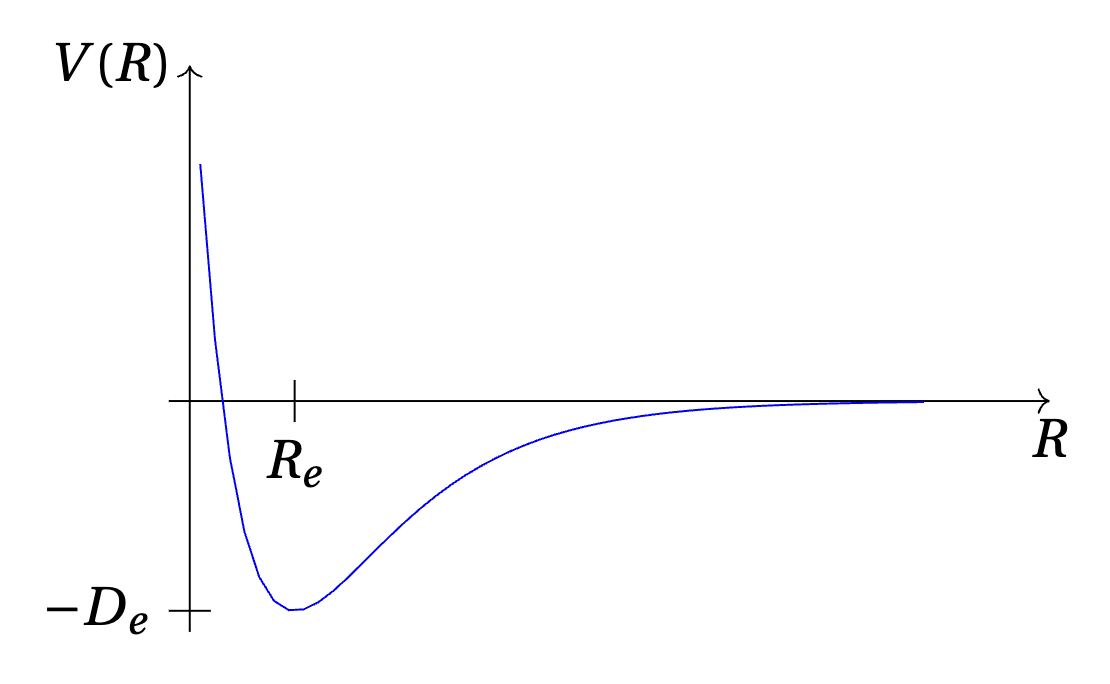
\includegraphics[width=0.8\linewidth]{fig/morse-potential.png}
    \caption{Morse Potential}
    \label{fig:morse_potential}
\end{figure}

\begin{equation}
    \label{eq:potential_bond_stretch}
    V(R) = D_{e} \left( e^{-2a(R-R_{e})} -2e^{-a(R-R_{e})} \right)
\end{equation}

\noindent โดยที่ $R_{e}$ คือระยะห่างระหว่างอะตอมที่สภาวะสมดุล เช่น ความยาวพันธะ ณ ตำแหน่งที่พลังงานศักย์ของ Morse Potentail
นั้นมีค่าน้อยที่สุด, $D_{e}$ คือความลึก (Depth) ของพื้นผิวศักย์ (Potentail Surface) ซึ่งก็คือพลังงานการแตกออกหรือการแยกตัว (Dissociation
Energy) และ $a$ คือพารามิเตอร์ที่อธิบายความกว้างของบ่อพลังงานศักย์อันนี้ นอกจากนี้ Morse Potential สามารถถูกเขียนได้ด้วยวิธีอื่น ๆ ได้อีกด้วย

หนึ่งในวิธีที่เราจะสามารถใช้ในการ Represent พันธะโควาเลนท์ก็คือการใช้โมเดลการสั่น Harmonic OSciallator แบบคลาสสิค
เช่น ถ้าเรามีอะตอม 2 อะตอมที่ถูกยึดเข้าด้วยกันด้วยสปริงที่มี Force Constant $k$ เราสามารถใช้ Taylor Expansion ในการอธิบาย Potential
Energy $V(R)$ ได้โดยการใช้ Dunham Expansion Parameter $Q = (\frac{R-R_{e}}{R_{e}})$ ดังนี้

\begin{equation}
    V(Q)
    =
    \underbrace{V(0)}_{\text {Zero level }}
    + \underbrace{V^{\prime}(0) Q}_{V^{\prime}(0)=0 \text { in the minimum }}
    + \underbrace{\frac{1}{2} V^{\prime \prime}(0) Q^2}_{\text {Harmonic term }}
    + \underbrace{\frac{1}{6} V^{(3)}(0) Q^3}_{\text {Anharmonicity }}
    + \underbrace{\frac{1}{24} V^{(4)}(0) Q^4 \ldots,}_{\text {Quartic term }}
\end{equation}

\noindent โดยที่เราไม่ต้องพิจารณา Zero Level ($V(0)$) ก็ได้ เพราะว่า Potential Energy Surface นั้นสามารถเปลี่ยนระดับพลังงาน%
ได้ด้วยค่าพลังงานคงที่ สำหรับเทอมที่เป็นเส้นตรง (Linear Term) ใน $Q$ นั้นมีค่าเท่ากับ 0 เนื่องจากว่า Gradient ของเทอมนี้นั้นเท่ากับ 0
ที่ตำแหน่ง Minimum ส่วนเทอมที่เป็น Quadratic Term กับ Cubic Term ใน $Q$ นั้นคือ Harmonic และ Anharmonic ของพื้นผิวศักย์ตามลำดับ
ถ้าหากว่าเราตัดเทอม Anharmonicity แล้วก็เทอมที่มีอันดับสูงกว่านี้ออกไปจาก Tarlor Expansion สิ่งที่เราจะได้นั้นก็คือการสั่นฮาร์โมนิคแบบ%
ดั้งเดิม (Classical Harmonic Oscillator) นั่นเอง

\begin{equation}
    V(Q)
    =
    \frac{k}{2} Q^{2} \quad \texttt{โดยที่} k \equiv V''(0)
\end{equation}

Taylor Expansion ของ Morse Potential นั้นเป็นหนึ่งโมเดลของพื้นผิวศักย์ที่สามารถอธิบายสถานะของระบบรอบ ๆ จุดต่ำสุด Minimum ได้
ซึ่งจะอธิบายได้ดีก็ต่อเมื่อเราทำการตัดหรือไม่พิจารณาเทอมที่มีอันดับสูงกว่า Harmonic Term ออกไป อย่างไรก็ตาม โมเดลนี้ก็มีจุดอ่อน ถ้าหากว่าเรา%
ดูกรณีที่อะตอมทั้งสองอะตอมนั้นมีระยะห่างกันมาก ๆ ซึ่งก็คือห่างกันอนันต์ $Q \rightarrow \infty$ จะทำให้พลังงานศักย์นั้นเข้าใกล้ค่าอนันต์ด้วย
$V(Q) \rightarrow \infty$ ซึ่งเงื่อนไขอันนี้ทำให้โมเดล Morse Potential นั้นอธิบาย Dissociation ได้ไม่ถูกต้อง แต่ถ้าหากว่าโมเดลอันนี้%
ถูกนำมาใช้ในการอธิบายระบบที่มีหลาย ๆ โมเลกุลและแต่ละโมเลกุลนั้นไม่ทำปฏิกิริยาต่อกัน พูดง่าย ๆ ก็คือไม่มีการสร้างพันธะ (Non-reacting)
เราจะพบว่าการที่เราทำการตัดเทอมที่มีอันดับสูงกว่า Harmomic ออกไปนั้นจะทำให้มันสามารถอธิบายพื้นผิวศักย์ได้อย่างสมเหตุสมผล

%----------------------------------------
\subsection{Angle Bending}
\idxen{Angle Bending}
%----------------------------------------

\begin{figure}[htbp]
    \centering
    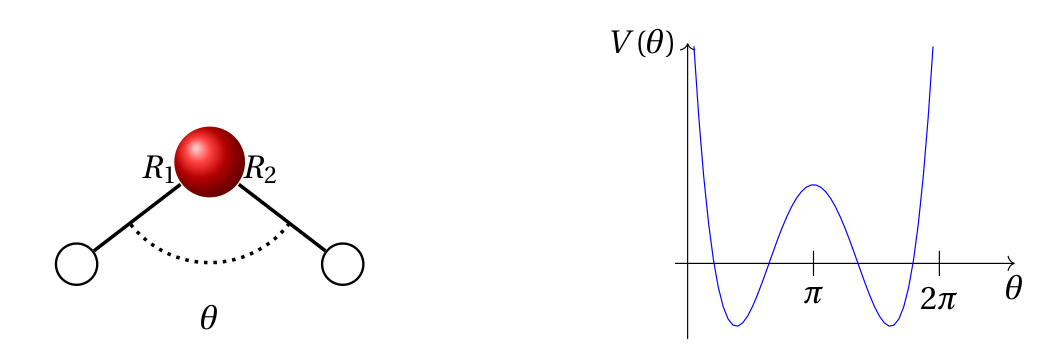
\includegraphics[width=0.8\linewidth]{fig/water-angle-bending.png}
    \caption{ซ้าย: โมเลกุลน้ำ, ขวา: Double Minimum Potential สำหรับมุมพันธะของโมเลกุลน้ำ}
    \label{fig:water_angle_bending}
\end{figure}

สำหรับการอธิบาย Angle Bending นั้นผมขอยกตัวอย่างโมเลกุลน้ำ \ce{H2O} ซึ่งมีมุมสมดุลคือ $\theta_{e}$ ระหว่างพันธะ \ce{O-H}
ซึ่งมีความยาวพันธะเท่ากับ 104.5 องศา เมื่อความยาวพันธะยืดออกนั้นเราสามารถใช้การประมาณแบบ Harmonic Oscillator เพื่ออธิบาย Angle
Bending ได้ ดังนี้

\begin{equation}
    V(\theta)
    =
    \frac{k_{\theta}}{2}
    (\theta - \theta_{e})^{2}
\end{equation}

\noindent ซึ่ง Approximation ด้านบนนี้สามารถนำมาใช้ได้เมื่อมุม $\theta$ นั้นเข้าใกล้กับมุมสมดุล $\theta_{e}$

ถ้าหากเราลองมาดูกรณีแปลก ๆ เช่น ถ้ามุมพันธะมีค่าเท่ากับ $\pi$ ซึ่งทำให้โมเลกุลน้ำนั้นเป็นเส้นตรง เราจะพบว่าพลังงานศักย์นั้นจะสูงมาก ๆ
และในความเป็นจริงนั้นแทบจะเป็นไปได้ยากมาก ๆ ที่โมเลกุลน้ำนั้นจะเป็นเส้นตรง (แต่ก็สามารถทำได้โดยการเพิ่มอุณหภูมิให้สูงมาก ๆ)

%----------------------------------------
\subsection{Dihedral Terms}
\idxen{Dihedral Terms}
%----------------------------------------

พารามิเตอร์อีกอันหนึ่งที่สำคัญมากในการอธิบายการเปลี่ยนแปลงของมุมพันธะและระนาบในโมเลกุลนั้นก็คือ Dihedral Angle หรือว่ามุมบิด
ซึ่งมุมบิดนี้ก็มี Potential Energy เป็นของตัวเองด้วยโดยมีสมการดังต่อไปนี้

\begin{equation}
    V(\omega)
    =
    \sum_{n} \frac{V_{n}}{2}
    \left(
    1 + \cos(n\omega - \gamma)
    \right)
\end{equation}

\noindent โดยที่ $n$ นั้นคือเลขจำนวนเต็มที่บ่งบอกถึงจำนวนคาบ เช่น $n = 2$ ก็คือมีคาบเท่ากับ 180 องศา หรือ $n = 3$ ก็คือมีคาบเท่ากับ
120 องศานั่นเอง, $V_{n}$ คือพลังงานศักย์การหมุน (Rotational Energy Barrier) และ $\gamma$ นั้นกำหนดว่ามุมที่มุมบิดนั้นมีค่าเท่ากับ
0 องศา

สมการที่ใช้ในการพลังงานศักย์ของ Dihedral Angle นั้นสามารถเขียนได้โดยการใช้ส่วนจริง (Real Part) ของการแปลงฟูเรียร์ ดังนี้

\begin{equation}
    V(\omega)
    =
    \sum_{n} C_{n} \cos(\omega)^{n}
\end{equation}


\begin{figure}[htbp]
    \centering
    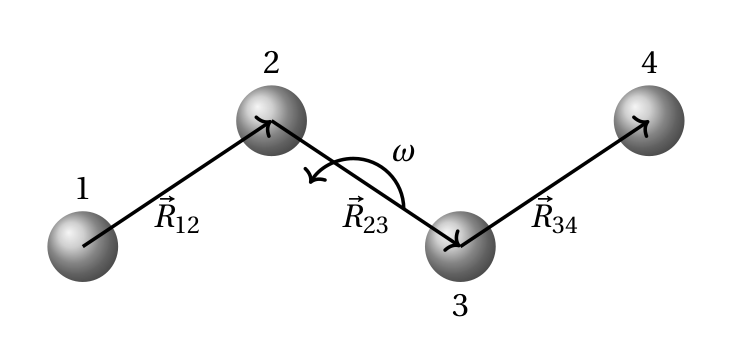
\includegraphics[width=0.8\linewidth]{fig/dihedral-angle.png}
    \caption{ซ้าย: โมเลกุลน้ำ, ขวา: Double Minimum Potential สำหรับมุมพันธะของโมเลกุลน้ำ}
    \label{fig:dihedral_angle}
\end{figure}

สำหรับโมเลกุลที่ควรจะต้องแบนราบหรือมีความเป็น Planar อยู่แล้วนั้น บางครั้งเราก็อยากที่จะเพิ่ม Constraint เข้าไปให้กับพื้นผิวศักย์ของโมเลกุล%
เพื่อทำให้โมเลกุลนั้นมีความเป็น Planar ซึ่งวิธีการเพิ่ม Constraint นั้นทำได้หลายวิธี หนึ่งในนั้นก็คือการใส่ Lagrangian Multipliers 
ในขณะที่เราทำการปรับค่าพลังงานของโมเลกุลให้มีค่าต่ำที่สุดหรือที่เราเรียกว่า Constrained Energy Minimization ซึ่งจะทำให้เราได้โมเลกุลที่%
มีพลังงานต่ำที่สุดที่สภาวะที่ถูก Constraint อยู่ด้วย จึงทำให้โมเลกุลนั้นถูกบังคับให้แบนราบหรือมีความเป็น Planar ตลอดเวลา นอกจากนี้ยังมีอีกวิธี%
ก็คือการเติมเทอมพลังงานพิเศษเข้าไปทื่อ ๆ เลยอีกเทอมนึง ซึ่งเทอมพลังงานพิเศษอันนี้ที่เราเติมเข้าไปนั้นมีชื่อเรียกว่า Energy Restraint หรือ 
Improper Torsion Term นั่นเอง ซึ่งมีหน้าตาดังนี้

\begin{equation}
    V(\omega)
    =
    k_{\omega}
    (1 - \cos 2\omega)
\end{equation}

\noindent โดยที่โมเลกุลนั้นจะถูกบังคับหรือถูกตรึงให้มีลักษณะที่ \textit{เกือบ} จะเป็นแบนราบอยู่ตลอดเวลาถ้าหากว่าค่า $k_{\omega}$ 
นั้นมีค่ามากพอ

%----------------------------------------
\subsection{Cross Terms}
\idxen{Cross Terms}
%----------------------------------------

เทอมสุดท้ายที่เรามักจะไม่ค่อยคุนชินกันเท่าไหร่เพราะว่ามักจะไม่ค่อยมีใครพูดถึงแม้แต่ในตำราต่างประเทศหลาย ๆ เล่มนั่นก็คือเทอมที่เรียกว่า Cross Term 
ซึ่งเทอมนี้จะถูกนำใส่เข้าไปใน Potential Energy Expression เพื่อใช้อธิบายการคู่ควบกัน (Coupling) ระหว่าง Two-bond Stretch 
หรือ Bond Stretch กับ Angle Bending Term โดยผมขอยกตัวอย่างด้วยโมเลกุลน้ำเหมือนเดิมครับ ถ้าหากเราพิจารณา Intermolecular Motion 
นั้นเราจะสามารถอธิบาย Motion อันนี้ได้โดยการใช้ Taylor Expansion รอบ ๆ ความยาวพันธะทั้งสองอัน ($R_{1}$ กับ $R_{2}$) และมุมพันธะ 
($\theta$) ดังนี้ 
   
\begin{align}
    V\left(R_1, R_2, \theta\right) 
    &= 
    V\left(R_{1,0}, R_{2,0}, \theta_0\right) 
        + \left.\left(R_1-R_{1,0}\right) \frac{\partial V}{\partial R_1}\right|_{R_{1,0}, R_{2,0}, \theta_0} \nonumber \\
    &+ \left.\left(R_2-R_{2,0}\right) \frac{\partial V}{\partial R_2}\right|_{R_{1,0}, R_{2,0}, \theta_0} \nonumber \\
    &+ \left.\left(\theta-\theta_0\right) \frac{\partial V}{\partial \theta}\right|_{R_{1,0}, R_{2,0}, \theta_0} 
        + \left.\frac{1}{2}\left(R_1-R_{1,0}\right)^2 
            \frac{\partial^2 V}{\partial R_1^2}\right|_{R_{1,0}, R_{2,0}, \theta_0} \nonumber \\
    &+ \left.\frac{1}{2}\left(R_2-R_{2,0}\right)^2 
        \frac{\partial^2 V}{\partial R_2^2}\right|_{R_{1,0}, R_{2,0}, \theta_0} 
        + \left.\frac{1}{2}\left(\theta-\theta_0\right)^2 
            \frac{\partial^2 V}{\partial \theta^2}\right|_{R_{1,0}, R_{2,0}, \theta_0} \\
    &+ \left.\left(R_1-R_{1,0}\right)\left(R_2-R_{2,0}\right) 
        \frac{\partial^2 V}{\partial R_1 \partial R_2}\right|_{R_{1,0}, R_{2,0}, \theta_0} \nonumber \\
    &+ \left.\left(R_1-R_{1,0}\right)\left(\theta-\theta_0\right) 
        \frac{\partial^2 V}{\partial R_1 \partial \theta}\right|_{R_{1,0}, R_{2,0}, \theta_0} \nonumber \\
    &+ \left.\left(R_2-R_{2,0}\right)\left(\theta-\theta_0\right) 
        \frac{\partial^2 V}{\partial R_2 \partial \theta}\right|_{R_{1,0}, R_{2,0}, \theta_0} + \ldots
\end{align}

\noindent โดยที่ 3 เทอมสุดท้ายนั้นคือ Coupling Terms อย่างไรก็ตาม โดยปกติแล้วเราไม่จำเป็นต้องใส่เทอม Coupling ทั้งหมดที่เรามี 
ซึ่งเทอม Coupling บางเทอมก็สำคัญ บางเทอมก็ไม่สำคัญซึ่งขึ้นอยู่กับโมเลกุล สำหรับโมเลกุลน้ำนั้นเทอม Coupling ที่สำคัญและควรจะต้องมีก็คือ 
Coupling Term ที่มาจาก Stretch Bond เพื่อที่ว่าจะสามารถอธิบาย Symmetric Stretch Coordinate ได้ ซึ่งมีสมการดังนี้

\begin{equation}
    Q_1-Q_{1,0} 
    =
    \left(R_1-R_{1,0}\right)+\left(R_2-R_{2,0}\right)
\end{equation}

\noindent และสามารถ Antisymmetric Stretch Coordinate ได้เช่นกัน ซึ่งมีสมการดังนี้

\begin{equation}
    Q_2-Q_{2,0} 
    = 
    \left(R_1-R_{1,0}\right)-\left(R_2-R_{2,0}\right)
\end{equation}

แล้วก็ในการรวม Crossing Term เข้าไปในสมการพลังงานศักย์เพื่อใช้อธิบายพื้นผิวศักย์ของโมเลกุลน้ำนั้น เราจะพบว่าพารามิเตอร์ที่ขึ้นอยู่กับชนิดของ%
อะตอมนั้น (เช่น $R_{1,0}$, $R_{2,0}$ และ $\theta_{0}$) นั้นไม่ได้เกี่ยวข้องหรือสอดคล้องกับ Equilibrium Geometry เลย 

%----------------------------------------
\subsection{สรุป Bonding}
%----------------------------------------

โดยสรุปแล้วเราเพิ่งได้ศึกษาเทอมของพลังงานต่าง ๆ ที่เรานำมาใช้ในการสร้าง Force Field เพื่อใช้ในการอธิบาย Covalent Bond ซึ่งประกอบไปด้วย%
เทอมดังต่อไปนี้ Bond Stretching, Angle Bending, Torsional Motion แล้วก็มีการรวมเทอมพิเศษเข้าไปด้วยซึ่งก็คือ Coupling Term 
และนอกจากนี้ยังมีเทอมอื่น ๆ อีกที่ผมไม่ได้พูดถึง เช่น เทอมพิเศษที่อธิบาย Hyperconjugation ซึ่งเป็นปรากฏการณ์ที่ $\pi$-conjugation 
นั้นส่งผลต่อการยืดหกของพันธะอย่างไรในโมเลกุล โดยเราสามารถแบ่งประเภทของเทอมเหล่านี้ออกเป็นคลาสได้ดังนี้

\begin{itemize}
    \item Class I: มีเพียงแค่ Harmonic Terms เท่านั้น ไม่มีการเติม Coupling Terms เข้าไป
    
    \item Class II: มี Anharmonic Terms และ Cross Terms 
    
    \item Class III: มีเทอมพื้นฐานทั้งหมดและมีการเพิ่มเทอมพิเศษ เช่น Huperconjugation เข้าไปด้วย
\end{itemize}

%----------------------------------------
\section{อันตรกิริยาระหว่างโมเลกุล}
\idxboth{อันตรกิริยาระหว่างโมเลกุล}{Intermolecular Interactions}
%----------------------------------------

ในหัวข้อที่ \ref{sec:md_ff_covalent_bond} เราได้ศึกษาอันตรกิริยาที่อยู่ภายในโมเลกุลไปแล้วนั่นก็คือพันธะโควาเลนท์ซึ่งเป็นอันกิริยาที่เกิดขึ้น%
ระหว่างอะตอม ในหัวข้อนี้ผู้อ่านจะได้ศึกษาอันตรกิริยาที่เกิดขึ้นระหว่างโมเลกุล เช่น อันตรกิริยาแบบอ่อน (Weak Interaction) ซึ่ง \enquote{อ่อน} 
ในที่นี้คือเทียบกับพันธะโควาเลนท์ ตัวอย่างเช่น Dispersion Interaction ที่เกิดขึ้นใน Liquid Argon, Hydrogen Bonding ที่เกิดขึ้นใน 
Liquid Water, หรือ Ion-Ion Interaction ที่เกิดขึ้นในสารละลายอิเล็กโทรไลต์ นอกจากนี้แล้วยังมีอันตรกิริยาอื่น ๆ ที่เกิดขึ้นระหว่างโมเลกุล%
ที่เราจะต้องพิจารณาด้วย เช่น อันตรกิริยาแบบไกล (Long-Range Interaction) ที่สามารถเกิดขึ้นได้ภายในโมเลกุลเดียวกันสำหรับโมเลกุลที่มี%
ขนาดใหญ่มาก ๆ ซึ่งพลังงานที่เกิดขึ้นจาก Long-Range Interaction นั้นก็เป็นอีกเทอมที่สำคัญมาก ๆ ที่ทำให้การจำลองโมเลกุลนั้นมีความถูกต้องมากขึ้น 
\idxboth{อันตรกิริยาระหว่างโมเลกุล!อันตรกิริยาแบบอ่อน}{Intermolecular Interactions!Weak Interaction}

ในหัวข้อนี้เราจะมาโพกัสพลังงานทั้งหมด 4 เทอมที่สำคัญซึ่งเป็นเทอมพลังงานที่เป็นตัวแทนของ Intermolecular Interaction ได้เป็นอย่างดีครับ

\begin{enumerate}[topsep=0pt,noitemsep]
    \setlength\itemsep{1em}
    \item พลังงานไฟฟ้าสถิตย์ (Electrostatic Energy): เป็นเทอมพลังงานที่อธิบายอันตรกิริยาระหว่างไอออนหรือโมเลกุลที่มีความมีขั้ว
    
    \item พลังงานเหนี่ยวนำ (Induction Energy): เป็นเทอมพลังงานที่อธิบายถึงการเปลี่ยนแปลงของความหนาแน่นของอิเล็กตรอนภายในโมเลกุล%
    ที่เกิดจากการถูก Polarized ด้วยสนามไฟฟ้าจากโมเลกุลรอบ ๆ ซึ่งส่งผลให้เกิดการเหนี่ยวนำ Electric Moment เช่น Induced Dipole 
    Moment 
    
    \item พลังงานผลักแบบใกล้ (Short-Range Repulsion Energy): เป็นเทอมพลังงานที่มาจากอันตรกิริยาแบบผลักระหว่างอิเล็กตรอนภาย%
    ซึ่งถูกอธิบายด้วย Pauli Exclusion Principle

    \item พลังงานกระจายตัว (Dispersion Energy): เป็นเทอมพลังงานที่อธิบายการ Correlation ของการเคลื่อนที่ของอิเล็กตรอน
\end{enumerate}

%----------------------------------------
\subsection{Electrostatic Interactions}
\idxth{อันตรกิริยาแบบไฟฟ้าสถิตย์}
\idxen{Electrostatic Interactions}
%----------------------------------------

%----------------------------------------
\subsection{Electronic Polarization}
\idxth{โพลาไรเซชั่นเชิงอิเล็กทรอนิกส์}
\idxen{Electronic Polarization}
%----------------------------------------

%----------------------------------------
\subsection{Dispersion และ Short-range Repulsion}
%----------------------------------------

%----------------------------------------
\subsection{Effective Force Field}
\idxth{สนามแรง!สนามแรงแบบมีประสิทธิภาพ}
\idxen{Force Field!Effective Force Field}
%----------------------------------------

%----------------------------------------
\subsection{สรุป Non-bonding}
%----------------------------------------

%----------------------------------------
\section{แรงระหว่างโมเลกุลจากกลศาสตร์ควอนตัม}
\idxth{แรงระหว่างโมเลกุลแบบควอนตัม}
\idxen{Quantum Intermolecular Forces}
%----------------------------------------

%----------------------------------------
\subsection{อนุพันธ์ลำดับที่หนึ่งของพลังงาน} 
\idxen{First-order Energy}
%----------------------------------------

%----------------------------------------
\subsection{อนุพันธ์ลำดับที่สองของพลังงาน}
\idxen{Second-order Energy}

%----------------------------------------

%----------------------------------------
\section{สมการของการเคลื่อนที่}
\idxboth{สมการของการเคลื่อนที่}{Equations of Motion}
%----------------------------------------

หัวใจสำคัญของ MD Simulations นั้นก็คืออันตรกิริยาระหว่างโมเลกุลนั่นก็คือ \enquote{แรง (Force)} โดยมีสมการสำคัญ 2 สมการที่ถือได้ว่า%
เป็นสมการหลักของ MD เลยก็ว่าได้ ดังนี้

\begin{equation}
    \label{eq:force_newton}
    m_{i}\bm{\ddot{r}}_{i} = \bm{f}_{i}
\end{equation}

\begin{equation}
    \label{eq:force_der_ener}
    \bm{f}_{i} = -\nabla_{i}V(\bm{r})
\end{equation}

\noindent สมการด้านบนนี้คือสมการการเคลื่อนที่ของนิวตัน (Newtonian Equation of Motion) สำหรับอะตอม $i$ โดยที่เป้าหมายของเรา%
นั้นก็คือการคำนวณแรง $\bm{f}$ ที่กระทำต่ออะตอมซึ่งสามารถคำนวณได้จากพลังงานศักย์ $V(\bm{r})$ นั่นเอง ส่วนเวกเตอร์ $\bm{r}$ นั้น%
ก็คือพิกัดคาร์ทีเซียนของตำแหน่งของอะตอม (นิวเคลียส) ทั้งหมดทุกอะตอมในโมเลกุลซึ่งเป็นพิกัดแบบ 3 มิติ

\begin{equation}
    \bm{r} = (\underbrace{r_{1,x}, r_{1,y}, r_{1,z}}_{\text{อะตอมตัวที่ 1}}, \dots,
    \underbrace{r_{N,x}, r_{N,y}, r_{N,z}}_{\text{อะตอมตัวที่ $N$}})
\end{equation}

โดยในการจำลอง MD นั้นจะเป็นการแก้สมการที่ \eqref{eq:force_newton} และ \eqref{eq:force_der_ener} พร้อม ๆ กันไปเป็นสเต็ป ๆ
ตลอดช่วงระยะเวลาที่ทำการจำลอง โดยระยะห่างระหว่างสเต็ปนั้นเรียกว่า Time Step $(\Delta t)$

%----------------------------------------
\section{ข้อจำกัดของ MD}
%----------------------------------------

วิธี MD นั้นก็เหมือนกับวิธีการจำลองทางคอมพิวเตอร์อื่น ๆ ที่มีข้อจำกัดทั้งในเชิงตัวโมเดลของวิธีเองกับในเชิงทรัพยากรที่ใช้ในการคำนวณ โดยข้อจำกัด%
ของ MD สามารถแบ่งออกได้เป็น 4 ข้อหลัก ๆ ดังนี้

\paragraph{1. Time Scale} สเกลเวลาหรือ Time Scale คือสเกลที่บอกถึงระดับของช่วงเวลาที่ใช้ในการอธิบายปรากฎการณ์หรือพฤติกรรมของโมเลกุล%
หรือระบบที่เราต้องการศึกษา เช่น การสั่นของพันธะโมเลกุลนั้นจะมี Time Scale ในระดับ Femtosecond ดังนั้น Time Scale ที่เหมาะสมสำหรับ%
การกำหนด Time Step นั่นจึงอยู่ที่ประมาณ 1 fs เพราะว่าถ้าหากเรากำหนด Time Step ที่กว้างหรือช้ากว่านี้เช่น 10 fs เราก็จะไม่สามารถติดตาม%
การสั่นของโมเลกุลได้เพราะว่าช่วงระยะเวลาที่ใช้ในการขยับหรือเปลี่ยนตำแหน่งของโครสร้างของโมเลกุลนั้นมากกว่าการสั่นของโมเลกุลหลายเท่า

สำหรับการจำลองเหตุการณ์หรือ Event ในการจำลอง MD นั้นเราควรจะต้องทราบถึงระยะเวลาที่เร็วที่สุดที่เหตุการณ์นั้นสามารถเกิดขึ้นได้ก่อน เช่น
การพับของโปรตีน (Protein Folding) นั้นจะใช้เวลาประมาณ 1 วินาที ดังนั้นถ้าหากเรากำนดให้ Time Step = 1 fs เราจะต้องทำการจำลอง
MD ประมาณ $10^{15}$ สเต็ปถึงจะสามารถจำลองการพับของโปรตีนได้ อย่างไรก็ตามในความเป็นจริงนั้นปรากฎการณ์ต่าง ๆ ของโมเลกุลที่เกิดขึ้นนั้น%
มักจะเกิดขึ้นในช่วงเวลาระดับ Microsecond $(\mu s)$

\paragraph{2. Length Scale} สเกลขนาดหรือ Length Scale คือสเกลที่บ่งบอกถึงขนาดของระบบที่ถูกจำลองซึ่ง Length Scale นี้จะแบ่ง%
ตามขนาดของระบบที่ใช้ในการศึกษา ถ้าหากเราต้องการที่จะศึกษาคุณสมบัติของระบบที่มีขนาดใหญ่ Length Scale ก็จะต้องสอดคล้องกับระบบด้วย
เช่น การจำลองโครงข่ายพอลิเมอร์ (Polymer) เพื่อให้มีความเหมาะสมและมีขนาดใหญ่ของระบบที่ใหญ่มากพอที่จะเป็นตัวแทนของระบบพอลิเมอร์%
ในธรรมชาติจริง ๆ

\paragraph{3. ความแม่นยำของแรงที่คำนวณได้} หัวใจสำคัญของ MD นั้นก็คือการคำนวณแรงที่เป็นอันตรกิริยาระหว่างอะตอมในโมเลกุล ถ้าหาก%
เราใช้วิธีการคำนวณแรงที่มีความแม่นยำสูงก็จะทำให้เราได้แรงที่มีความถูกต้องมาก แต่วิธีการที่มีความแม่นยำสูงนั้นมักจะต้องแลกมาด้วยการคำนวณที่%
สิ้นเปลือง ดังนั้นเรามักจะทำการ Trade-off หรือชั่งน้ำหนักระหว่างการเลือกวิธีในการคำนวณแรงและความสิ้นเปลืองของวิธีนั้น ๆ เพราะอย่าลืมว่า%
เราต้องคำนวณแรงทุก ๆ สเต็ปของการจำลอง MD

%----------------------------------------
\section{ขั้นตอนการจำลอง MD}
%----------------------------------------

การจำลอง MD นั้นโดยปกติแล้วประกอบไปด้วยขั้นตอนดังต่อไปนี้

\paragraph{1. เลือกโมเดล}

\paragraph{2. เตรียมโครงสร้างเริ่มต้น}

\paragraph{3. รันการจำลอง MD}

\paragraph{4. วิเคราะห์ผลการจำลอง MD}

\paragraph{5. คำนวณคุณสมบัติอื่น ๆ เพิ่มเติม}

%----------------------------------------
\section{การจำลอง MD ด้วยเทคนิค Enhanced Sampling}
%----------------------------------------

%----------------------------------------
\section{การวิเคราะห์ผลการจำลอง MD}
%----------------------------------------

%----------------------------------------
\section{แบบฝึกหัด}
%----------------------------------------
